\begin{frame}
    \frametitle{Single Slab Hierarchy}
    \begin{block}{The single slab hierarchy (SSH)}
        \textbf{Иерархия одиночных пластин} - полное k-арное дерево BVH, которое хранится в массиве
        и индексируется как heap.
        Каждый узел либо листовой, либо имеет k дочерних.
        Это способ разделения BV надвое одной пластиной,
        в результате чего получается k-ичное дерево.
    \end{block}

    Принцип, используемый для этого компактного представления BVH:
    \begin{itemize}
        \item
            \textbf{Сокращение информации}, которая хранится для каждого BV
    \end{itemize}

\end{frame}

\begin{frame}
    \frametitle{Bounding Plane Adjustment}
    \framesubtitle{Single Slab Hierarchy}
    Чтобы не оставлять пустот в BVH, для каждого дочернего узла мы подбираем
    свою ось вдоль которой разместить splitting plane (single slab).

    Значит, помимо координаты по оси нашей splitting plane, для каждого узла нужно
    хранить выбранную ось (как флаг).
    \begin{figure}
        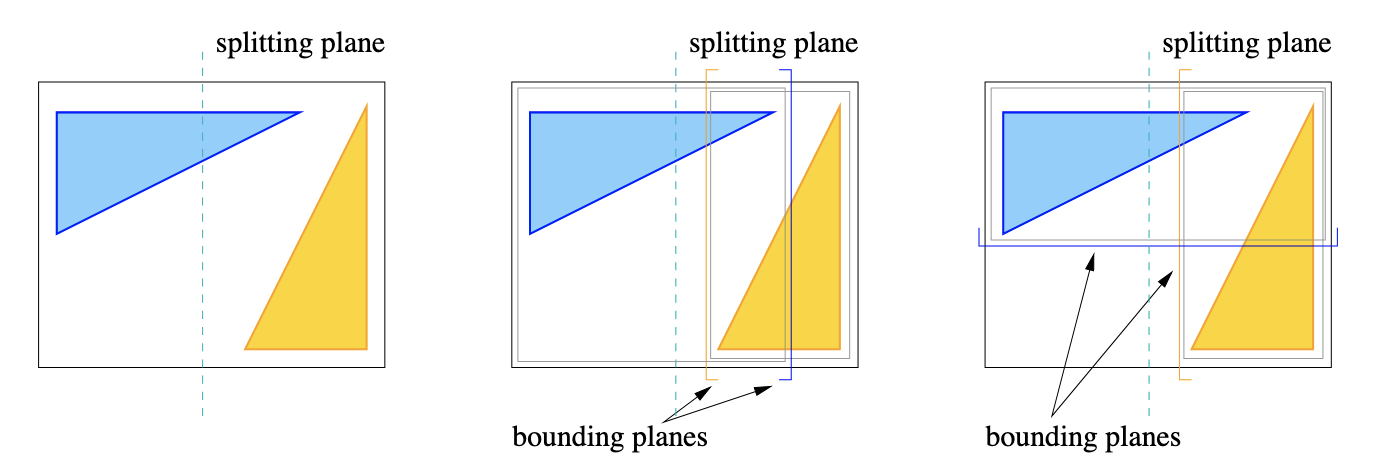
\includegraphics[keepaspectratio, width=\textwidth]{res/splitting_ssh.png}
    \end{figure}
\end{frame}

\begin{frame}[fragile]
    \frametitle{Структура Узла}
    \framesubtitle{Single Slab Hierarchy}

    \begin{semiverbatim}
        #pragma align(8)
        struct SSHNode \{
            float plane;
            union \{
                int firstChildNodeID; //inner nodes
                int firstTriangleID; //leaf nodes
                // bit 0..1: x/y/z/leaf
                // bit 2: left/right interior
                // bit 3..4: traversal axis
            \}
        \};
    \end{semiverbatim}
    Заняв 5 битов флагами у нас остается 27 битов (от int32),
    чтобы сохранить индекс.
    Таким образом можно закодировать до 134 мил. примитивов.

\end{frame}

\begin{frame}[fragile]
    \frametitle{Построение}
    \framesubtitle{Single Slab Hierarchy}

    \begin{lstlisting}[language=C++,basicstyle=\ttfamily,keywordstyle=\color{blue}]
void createSSH(TriangleList tris, AABB parent,
                SSHNode& node) {
    AABB bounds(tris); // bounding box
    float bestSurface = HUGE_VAL;
    int bestSide = 0;
    for (Side side : make_sides(bounds)) {
        AABB temp(parent);
        temp.side = side;
        if (surface(temp) < bestSurface) {
            bestSurface = surface(temp);
            bestSide = side;
        }
    }
    ...

    \end{lstlisting}

\end{frame}

\begin{frame}[fragile]
    \frametitle{Построение (продолжение)}
    \framesubtitle{Single Slab Hierarchy}
    \begin{lstlisting}[language=C++,basicstyle=\ttfamily,keywordstyle=\color{blue}]
    ...
    node.boundingPlane = boudns.bestSide;

    if (tris.size() < n) {
        createLeafNode(); return; }

    TriangleList leftTris, rightTris;
    subdivide(tris, leftTris, rightTris); // SAH
    parent.bestSide = boudns.bestSide;

    int childID = node.firstChildNodeID;
    createSSH(leftTris, parent, childID);
    createSSH(rightTris, parent, childID + 1);
}
    \end{lstlisting}
\end{frame}

\begin{frame}[fragile]
    \frametitle{Обход SSH}
    \framesubtitle{Single Slab Hierarchy}
    \begin{lstlisting}[language=C++,basicstyle=\ttfamily,keywordstyle=\color{blue}]
bool intersectSSH(Ray& ray, mask reverse[3],
        SSHNode* node, float& t_hit,
        float& t_near, float& t_far) {

    // 1. Calculate the distance to its BP
    int axis = node->getSlabAxis();
    float t = (node->plane - ray.origin[axis])
        / ray.dir[axis];
    // 2. Compare it to the active ray segment
    if (node->geometryIsLeft()) {
        t_near = (reverse[axis] | (t <= t_near))
            ? t_near : t;
        t_far  = (reverse[axis] & (t < t_far))
            ? t : t_far;
    ...

    \end{lstlisting}
\end{frame}

\begin{frame}[fragile]
    \frametitle{Обход SSH (продолжение)}
    \framesubtitle{Single Slab Hierarchy}

    \begin{lstlisting}[language=C++,basicstyle=\ttfamily,keywordstyle=\color{blue}]
    ...
    } else {
        t_near = (reverse[axis] & (t > t_near))
            ? t_near : t;
        t_far  = (reverse[axis] | (t >= t_far))
            ? t : t_far;
    }

    if ((t_near > t_far) || (t_near > t_hit)) {
        return false;
    }

    if (node->isLeaf()) { ... } else { ... };
}
    \end{lstlisting}
\end{frame}

\begin{frame}
    \frametitle{Extension to dynamic scenes}
    \framesubtitle{Single Slab Hierarchy}
    \begin{block}{Skinned meshes}
        Можно применить простой bottom-up подход,
        используя тривиальные min/max операции для адаптации границ узлов.
        Структура иерархии остается неизменной.

        Этого достаточно для большинства когерентных анимаций.
    \end{block}

    \begin{block}{Arbitrary movements}
        Можно параллельно перестраивать SSH. Как только построение будет завершено - сделать замену.
    \end{block}

\end{frame}

\begin{frame}[t]
    \frametitle{Плюсы и минусы}
    \framesubtitle{Single Slab Hierarchy}
    \textbf{Достоинства}:
    \begin{itemize}
        \item
            Сжатие 75\%
        \item
            Подходит для интерактивного рейтрейсинга
        \item
            Возможность адаптировать под динамические сцены
        \item
            Более легкий алгоритм траверса (в 6 раз быстрее чем пересекать с AABB)
        \item
            Не изменена структура самого дерева - изменено только представление узлов
        \item
            Сравним по скорости с обычным AABB BVH
    \end{itemize}
    \textbf{Недостатки}:
    \begin{itemize}
        \item
            Немного дольше строить
        \item
            В два раза больше узлов посещается при обходе по сравнению с AABB BVH
        \item
            В среднем на один треугольник на луч пересекается больше
    \end{itemize}
\end{frame}

\begin{frame}[t]
    \frametitle{Результаты}
    \framesubtitle{Single Slab Hierarchy}
    \begin{columns}
        \column{0.7\textwidth}
        \begin{itemize}
            \item
                $N_T$: avg of traversed nodes per ray
            \item
                $N_I$: avg of ray-object intersections per ray
            \item
                $T_C$: total time needed for \textbf{construction}
            \item
                $T_R$: total time needed for \textbf{traversal}
            \item
                $s(T_R)$: speedup achieved by the SSH with respect to the BVH
            \item
                $Mem$: memory usage of the AS in megabytes, excluding the triangle data
        \end{itemize}
        \column{0.5\textwidth}
        \begin{figure}
            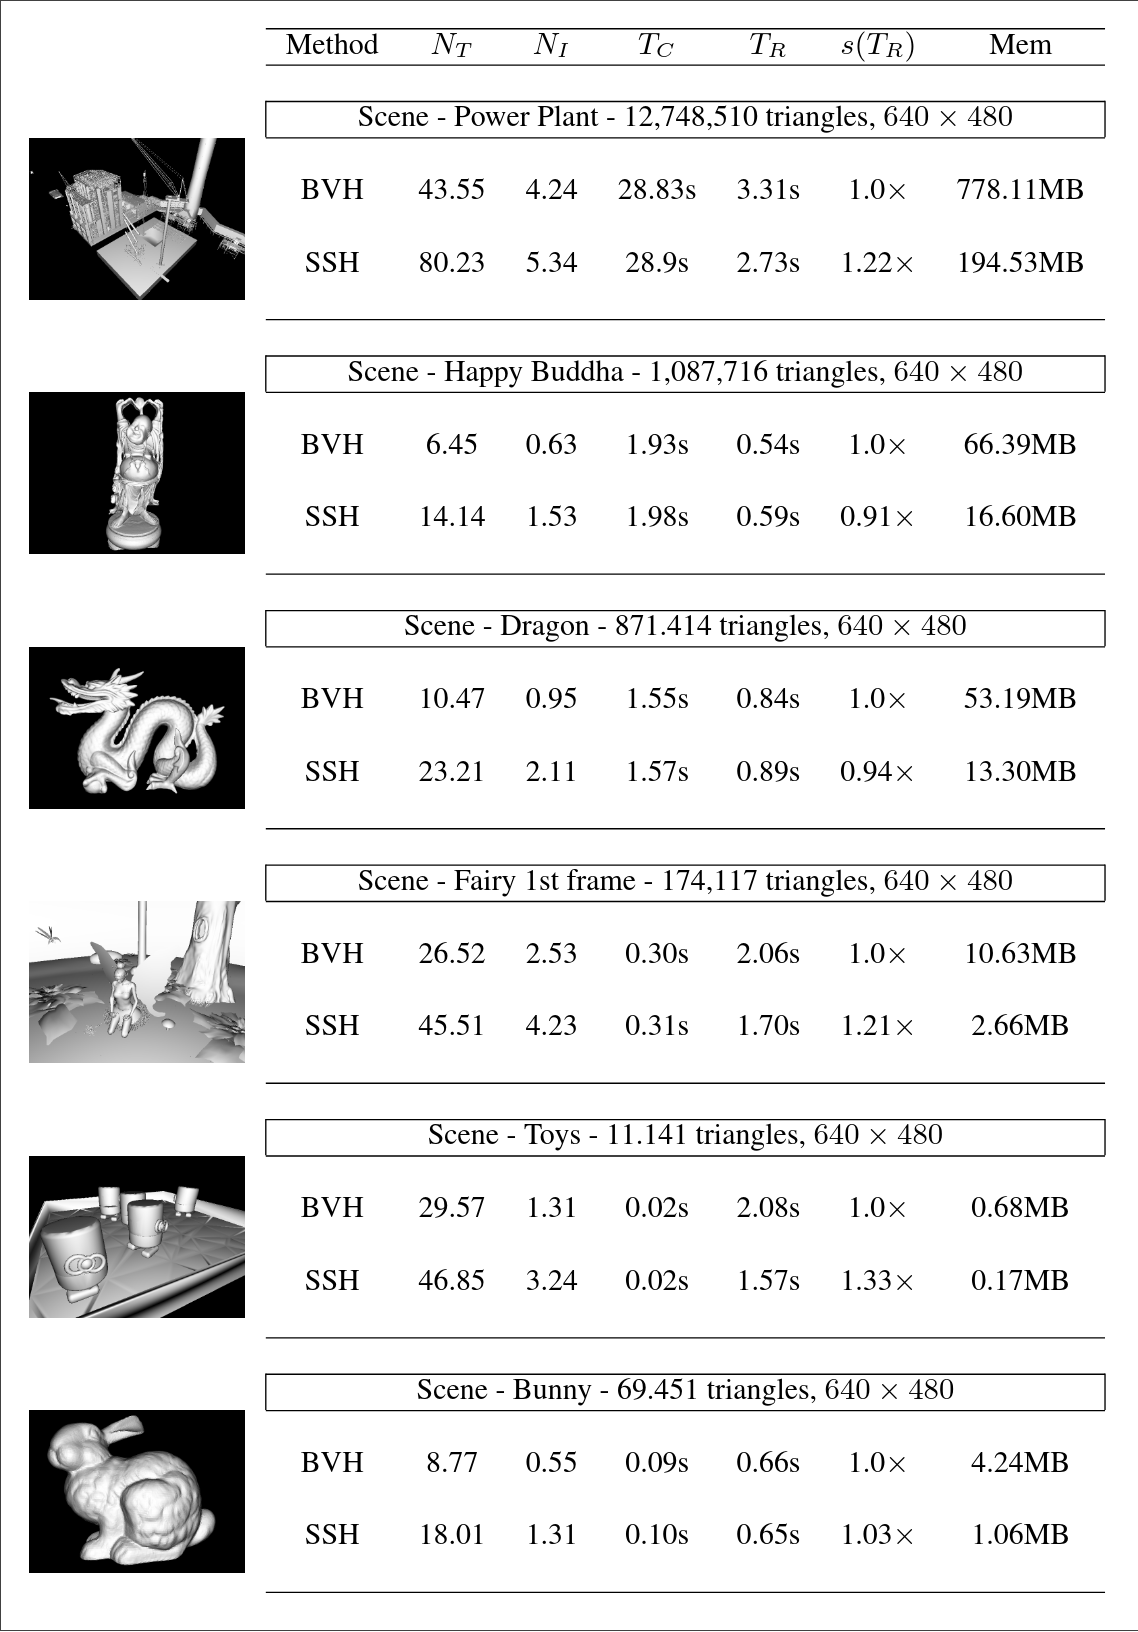
\includegraphics[keepaspectratio, height=.75\textheight]{res/results_ssh.png}
        \end{figure}
    \end{columns}

\end{frame}

